\documentclass[10pt,final,a4paper,oneside,onecolumn]{article}

%%==========================================================================
%% Packages
%%==========================================================================
\usepackage[a4paper,left=3.5cm,right=3.5cm,top=3cm,bottom=3cm]{geometry} %% change page layout; remove for IEEE paper format
\usepackage[T1]{fontenc}                        %% output font encoding for international characters (e.g., accented)
\usepackage[cmex10]{amsmath}                    %% math typesetting; consider using the [cmex10] option
\usepackage{amssymb}                            %% special (symbol) fonts for math typesetting
\usepackage{amsthm}                             %% theorem styles
\usepackage{dsfont}                             %% double stroke roman fonts: the real numbers R: $\mathds{R}$
\usepackage{mathrsfs}                           %% formal script fonts: the Laplace transform L: $\mathscr{L}$
\usepackage[pdftex]{graphicx}                   %% graphics control; use dvips for TeXify; use pdftex for PDFTeXify
\usepackage{array}                              %% array functionality (array, tabular)
\usepackage{upgreek}                            %% upright Greek letters; add the prefix 'up', e.g. \upphi
\usepackage{stfloats}                           %% improved handling of floats
\usepackage{multirow}                           %% cells spanning multiple rows in tables
%\usepackage{subfigure}                         %% subfigures and corresponding captions (for use with IEEEconf.cls)
\usepackage{subfig}                             %% subfigures (IEEEtran.cls: set caption=false)
\usepackage{fancyhdr}                           %% page headers and footers
\usepackage[official,left]{eurosym}             %% the euro symbol; command: \euro
\usepackage{appendix}                           %% appendix layout
\usepackage{xspace}                             %% add space after macro depending on context
\usepackage{verbatim}                           %% provides the comment environment
\usepackage[dutch,USenglish]{babel}             %% language support
\usepackage{wrapfig}                            %% wrapping text around figures
\usepackage{longtable}                          %% tables spanning multiple pages
\usepackage{pgfplots}                           %% support for TikZ figures (Matlab/Python)
\pgfplotsset{compat=1.14}						%% Run in backwards compatibility mode
\usepackage[breaklinks=true,hidelinks,          %% implement hyperlinks (dvips yields minor problems with breaklinks;
bookmarksnumbered=true]{hyperref}   %% IEEEtran: set bookmarks=false)
%\usepackage[hyphenbreaks]{breakurl}            %% allow line breaks in URLs (don't use with PDFTeX)
\usepackage[final]{pdfpages}                    %% Include other pdfs
\usepackage[capitalize]{cleveref}				%% Referensing to figures, equations, etc.
\usepackage{units}								%% Appropriate behavior of units
\usepackage[utf8]{inputenc}   				 	%% utf8 support (required for biblatex)
\usepackage{csquotes}							%% Quoted texts are typeset according to rules of main language
\usepackage[style=ieee,doi=false,isbn=false,url=false,date=year,minbibnames=15,maxbibnames=15,backend=biber]{biblatex}
%\renewcommand*{\bibfont}{\footnotesize}		%% Use this for papers
\setlength{\biblabelsep}{\labelsep}
\bibliography{../../bib}

%%==========================================================================
%% Define reference stuff
%%==========================================================================
\crefname{figure}{Figure}{Figures}
\crefname{equation}{}{}

%%==========================================================================
%% Define header/title stuff
%%==========================================================================
\newcommand{\progressreportnumber}{29}
\renewcommand{\author}{Erwin de Gelder}
\renewcommand{\date}{2020, April 7}
\renewcommand{\title}{Performance assessment of automated vehicles using real-world driving scenarios}

%%==========================================================================
%% Fancy headers and footers
%%==========================================================================
\pagestyle{fancy}                                       %% set page style
\fancyhf{}                                              %% clear all header & footer fields
\fancyhead[L]{Progress report \progressreportnumber}    %% define headers (LE: left field/even pages, etc.)
\fancyhead[R]{\author, \date}                           %% similar
\fancyfoot[C]{\thepage}                                 %% define footer

\begin{document}
	
\begin{center}
	\begin{tabular}{c}
		\title \\ \\
		\textbf{\huge Progress report \progressreportnumber} \\ \\
		\author \\ 
		\date
	\end{tabular}
\end{center}

\section{Previous meeting minutes}

\begin{itemize}
	\item We discussed the potential journals for publications of articles.
	\item I presented some ideas for the generation of test cases for the assessment of automated vehicles.
\end{itemize}

\section{Summary of work}

I mainly worked on a methodology for generating test cases. In short, the method to generate scenarios is as follows:

\begin{enumerate}
	\setcounter{enumi}{-1}
	\item Start: A given scenario category for which test cases are to be generated and observed scenarios from the same scenario category. The data of the observed scenarios are using the estimate the likelihoods of the actors, activities, initial conditions, and parameters.
	\item Determine the actor(s).
	\item Determine the initial activities of the actor(s).
	\item Determine the initial conditions. Note that this might depend on the actors and the initial activities.
	\item Determine the parameters of the initial activities. Note that these parameters might depend on the actor(s), the initial activities, and the initial conditions.
	\item If we reached the end of the test case, then stop. \label{sec:check stop}
	\item Determine next activity. The type of activity might depend on the actors, the previous activities, and the previous parameters.
	\item Determine the parameters of the next activity. These parameters might depend on the actors, the previous activities, and the previous parameters. After this step, go to step \ref{sec:check stop}.
\end{enumerate}

In this work in which I want to describe this method, I would like to mention to following:
\begin{itemize}
	\item For determining the activities, we can make use of the tags that are used to label the data of the observed scenarios. Using the tags, the probabilities of the initial activities can be estimated as well as the ``transition probabilities'', i.e., the probability to go from activity A to activity B.
	\item The initial conditions and the parameters might depend on the initial activities of the actors. One way to determine this is to apply statistical tests, such as the Kolmogorov-Smirnov test. However, there are situations in which these tests fail. Because for our purpose, we will use Kernel Density Estimation (KDE) to estimate the probability density functions of the parameters and the initial conditions and, therefore, we can also use these KDE to determine whether the initial conditions and the parameters depend on the initial activities and the actors. Due to limited time, I will not describe all details here, but loosely said, I estimate for both cases (in case there is a dependence and in case there is no dependence) the probability density functions and based on the leave-one-out-cross-validation score, I select the best case.
	\item As explained in the previous report, to increase the accuracy of the estimated probability function near the tails, a \emph{sample-point} estimator can be used \autocite{sain2002multivariate}.
	\item As explained in the previous report, for estimating the probability function for multivariate data, a pair-copula construction can be used \autocite{aas2009paircopula,czado2010paircopula,nagler2016evading}.
\end{itemize}

In the last weeks, I worked on the code for a case study in which I can apply the above method. This is still \emph{work in progress}, so I hope to tell more about that next time.

\section{Future plans}

In \cref{fig:planning}, the updated planning is shown. The only change is that the FISITA conference is postponed for a year. 

\begin{figure}[t]
	\centering
	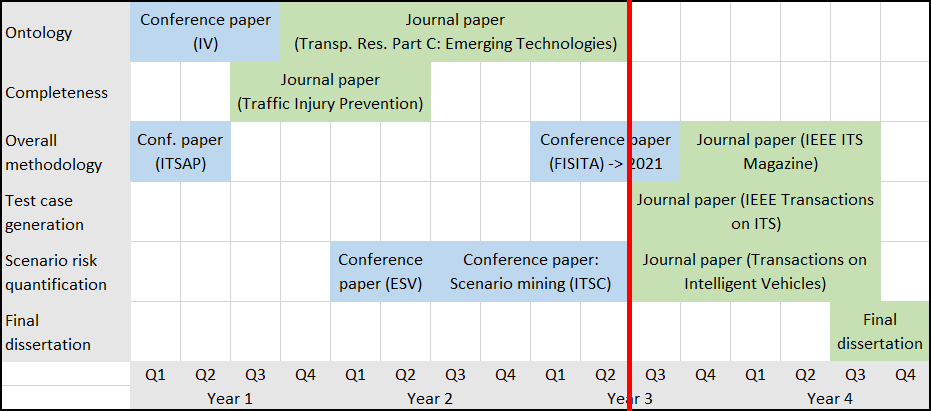
\includegraphics[width=\linewidth]{planning.png}
	\caption{Proposed planning at the time of this report. The red line indicated the time when writing this report.}
	\label{fig:planning}
\end{figure}

For the coming weeks, I will work on:
\begin{itemize}
	\item The code for the test case generation. 
	\item Describing in more detail the method for the test case generation.
	\item Currently, I do not have a project for the scenario risk quantification. In the last weeks, I had some internal discussions to further work on this inside a project, so I hope to tell more about this during the next meeting.
\end{itemize}


\printbibliography

%\clearpage
%\includepdf[pages=-,pagecommand={},width=\paperwidth]{../../""/.pdf}

\end{document}